\documentclass[12pt,letterpaper]{article}
\usepackage{tikz}
\usepackage{graphicx}
\usetikzlibrary{shapes,arrows}
\title{CS146 - Homework 6}
\author{Frank Mock}
\begin{document}
\maketitle
\section*{6.7 a.}


For a binary tree with \textbf{n} elements the for loop in the buildheap method starts at position $\frac{n}{2}$ and counts down to zero. Each of these $\frac{n}{2}$ elements may have to swap with a child. It takes two comparisons for each swap (one to find the smaller child and one to compare that child to the parent). Each swap may cause a need to restore heap order down the tree, this depends on the height of the parent node. Therefore each of the $\frac{n}{2}$ nodes potentially may have to perform 2 comparisons times it's height in the tree.

For example: For a complete binary tree with $n = 15$ elements, buildheap starts at position $\frac{n}{2} = \frac{15}{2} = 7$\\
Since we have 7 nodes, there are $2^2$ elements with a height of 1, $2^1$ elements with a height of 2, and $2^0$ elements(root) with a height of 3. The sum of the heights is therefore 11. The text book gives an equation for this as: $Sum_H = N - b(N)$ where  $b(N)$ is the number of 1s in the binary representation on N. To verify this I will use the number 15 from the previous example. There are four 1s in the binary representation. So plugging in $N = 15$, $15 - 4 = 11$. Since the number of comparisons is 2 times the sum of the heights of all the nodes, we get 22 comparisons for this example.\\\\
The question asks to prove that for binary heaps, \textbf{buildHeap} does at most $2N-2$ comparisons. So they are making $2N-2$ an upper bound on the number of comparisons. Using our previous example of a tree with 15 elements we can see that this is correct. $2(15) - 2 = 28$ which is close to , but greater than 22. Now I will attempt a formal proof:\\\\
\newpage
\textbf{Proof by induction:}\\
This proof will prove that $2(N - b(N))$ is $O(2N - 2)$, that is $2(N-b(N))$ is upper bounded by $2N - 2$\\\\
To prove: $2(N - b(N)) <= 2N - 2$\\ \scriptsize where b(N) is the number of 1s in the binary representation of N \small\\\\
Base Case for $N = 1$\hspace*{.25 in} $2(1 - 1) <= 2(1) - 2$\\
\hspace*{2.25 in}$0 = 0$ \hspace{.25 in} holds for N = 1\\\\
Assume it is also true for an arbitrarily chosen integer $k$ with $k >= 1$.\\
$2(k - b(k)) <= 2k - 2$ \hspace*{.5 in} Inductive Hypothesis\\\\
Show that it is also true for $k + 1$\\\\
$2(k+1 - b(k+1)) <= 2k+1 - 2$\\\\
$2k+2 - 2b(k+1)) <= 2k - 1$ \hspace*{.5 in} using basic algebra on both sides\\\\
$-2b(k+1)<=-3$ \hspace*{.5 in} using basic algebra on both sides\\\\
$b(k+1)>=\frac{3}{2}$ \hspace*{.5 in} division by negative 2 flips the inequality\\\\
Which is true since computer science uses integer division. End Proof\\
\section*{6.7 b.}
We can use a binomial queue structure. Insertions take constant time on average. A binomial queue is a set of heaps where each heap has a size of a power of two and no two heaps are the same size. So for this problem, we are asked to show that a heap of eight elements can be constructed with only eight comparisons. Since each heap in the binomial queue is a power of two we can look at the binary representation of 8 to see the structure of the binomial heap after eight inserts. 1000 is 8 in binary. Since there is only a 1 at the MSB place, this binomial queue will consist of a single heap of size $2^3$. Each insert is the same as merging a single element heap with the existing heap forest. Just like adding 1 to a binary number at the LSB place a carry over may occur.\\\\
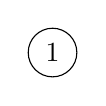
\begin{tikzpicture}
\tikzstyle{every node}=[circle,draw]
\node {1};
\end{tikzpicture} First number is inserted(no comparisons).\\\\
\begin{tabular}{ |l|l|l|l| }
   \hline
   $2^3$  & $2^2$  & $2^1$  & $2^0$ \\ \hline
    0 & 0 & 0 & 1 \\
   \hline
 \end{tabular} One heap with a single element\\\\
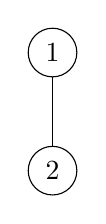
\begin{tikzpicture}
\tikzstyle{every node}=[circle,draw]
\node {1}
	child{node{2}};
\end{tikzpicture} Second number is inserted(one comparison).\\\\
\begin{tabular}{ |l|l|l|l| }
   \hline
   $2^3$  & $2^2$  & $2^1$  & $2^0$ \\ \hline
    0 & 0 & 1 & 0 \\
   \hline
 \end{tabular} One heap with two elements\\\\
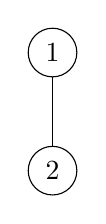
\begin{tikzpicture}
\tikzstyle{every node}=[circle,draw]
\node {1}
	child{node{2}};
\end{tikzpicture}
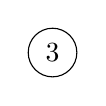
\begin{tikzpicture}
\tikzstyle{every node}=[circle,draw]
\node {3};
\end{tikzpicture}Third insert. Binomial queue is now two heaps of sizes $2^0$ \& $2^1$\\\\
\begin{tabular}{ |l|l|l|l| }
   \hline
   $2^3$  & $2^2$  & $2^1$  & $2^0$ \\ \hline
    0 & 0 & 1 & 1 \\
   \hline
 \end{tabular} No comparison. New element free to use size $2^0$\\\\
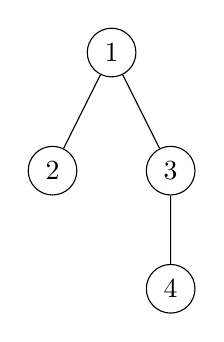
\begin{tikzpicture}
\tikzstyle{every node}=[circle,draw]
\node {1}
	child {node{2}}
	child {node{3} child{node{4}}};
\end{tikzpicture}Fourth insert. Binomial queue is a single heap of size $2^2$
\begin{tabular}{ |l|l|l|l| }
   \hline
   $2^3$  & $2^2$  & $2^1$  & $2^0$ \\ \hline
    0 & 1 & 0 & 0 \\
   \hline
 \end{tabular}\\Two comparisons which is the same as the number of carry overs when adding 1 to binary 011\\\\
\newpage
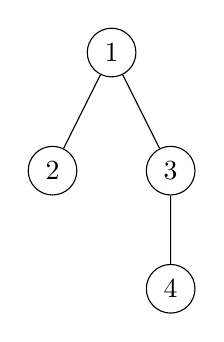
\begin{tikzpicture}
\tikzstyle{every node}=[circle,draw]
\node {1}
	child {node{2}}
	child {node{3} child{node{4}}};
\end{tikzpicture}
\hspace*{.25 in}
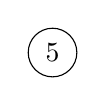
\begin{tikzpicture}
\tikzstyle{every node}=[circle,draw]
\node {5};
\end{tikzpicture}\\\\Fifth insert. Binomial queue is two heaps of sizes $2^2$ and $2^0$\\
\begin{tabular}{ |l|l|l|l| }
   \hline
   $2^3$  & $2^2$  & $2^1$  & $2^0$ \\ \hline
    0 & 1 & 0 & 1 \\
   \hline
 \end{tabular} No comparisons. $5^{th}$ insert is free to use heap size $2^0$\\\\\\
 Total comparisons so far is 3.\\\\\\
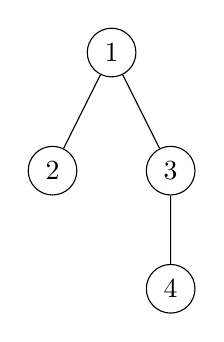
\begin{tikzpicture}
\tikzstyle{every node}=[circle,draw]
\node {1}
	child {node{2}}
	child {node{3} child{node{4}}};
\end{tikzpicture}
\hspace*{.25 in}
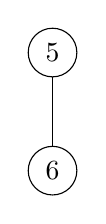
\begin{tikzpicture}
\tikzstyle{every node}=[circle,draw]
\node {5}
	child{node{6}};
\end{tikzpicture}\\\\Sixth insert. Binomial queue is two heaps of sizes $2^2$ and $2^1$\\
\begin{tabular}{ |l|l|l|l| }
   \hline
   $2^3$  & $2^2$  & $2^1$  & $2^0$ \\ \hline
    0 & 1 & 1 & 0 \\
   \hline
 \end{tabular}\\One comparison - same as number of carry overs when adding 1 to binary 101.\\\\
Total comparisons so far is 4.
\newpage
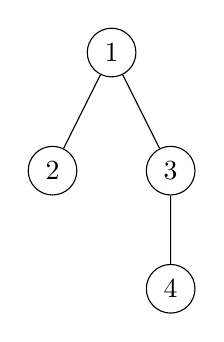
\begin{tikzpicture}
\tikzstyle{every node}=[circle,draw]
\node {1}
	child {node{2}}
	child {node{3} child{node{4}}};
\end{tikzpicture}
\hspace*{.25 in}
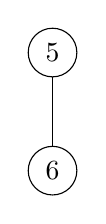
\begin{tikzpicture}
\tikzstyle{every node}=[circle,draw]
\node {5}
	child{node{6}};
\end{tikzpicture}
\hspace*{.25 in}
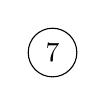
\begin{tikzpicture}
\tikzstyle{every node}=[circle,draw]
\node {7};
\end{tikzpicture}\\Seventh insert. Binomial queue is three heaps of sizes $2^2$, $2^1$ and $2^0$\\
\begin{tabular}{ |l|l|l|l| }
   \hline
   $2^3$  & $2^2$  & $2^1$  & $2^0$ \\ \hline
    0 & 1 & 1 & 1 \\
   \hline
 \end{tabular}\\No comparison - $7^{th}$ insert free to use heap size $2^0$.\\\\\\
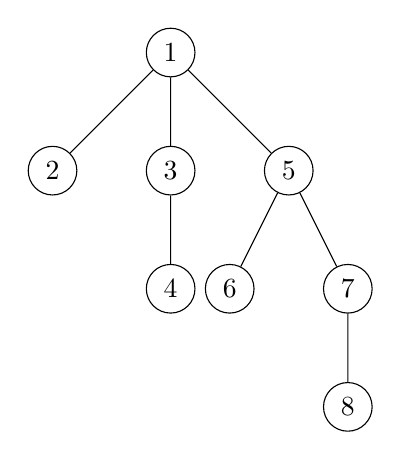
\begin{tikzpicture}
\tikzstyle{every node}=[circle,draw]
\node {1}
	child {node{2}}
	child {node{3} child{node{4}}}
	child {node{5} child{node{6}} child{node{7} child{node{8}}}};
\end{tikzpicture}\\\\
Eighth insert. Binomial queue is a single heap of size $2^3$
\begin{tabular}{ |l|l|l|l| }
   \hline
   $2^3$  & $2^2$  & $2^1$  & $2^0$ \\ \hline
    1 & 0 & 0 & 0 \\
   \hline
 \end{tabular}\\
The $8^{th}$ insert causes three comparisons which is the same as the number of carry overs when adding 1 to the binary number 111.\\\\
Total number of comparisons is 7 (one per edge of heap).\\
I showed its possible in 7 comparisons. Hopefully, there is not a comparison I did not consider.
\newpage
\section*{6.10 a.}
\textit{Algorithm to find all nodes less than some value X, in a binary heap.}\\
My algorithm would use a preorder traversal comparing the root of each subtree to X. If the root is greater than X, there is no need to search any lower levels of the tree:\\\\
public int a[ ] \textbf{findAllLess}(int X)\\
int a[ ] //create an array to store numbers that are less\\
\textbf{if} the tree is empty\\
\hspace*{.25 in}return\\
\textbf{else}\\
\hspace*{.25 in}\textbf{if} the root $<$ X\\
\hspace*{.5 in}add X to array\\
\hspace*{.5 in}findAllLess the left subtree\\
\hspace*{.5 in}findAllLess the right subtree\\\\
return the array of values
\section*{6.14}
The parent of each element \textit{i} in a d-heap is at position:\\ $\lfloor(i + (d - 2))/d\rfloor$\\\\
The children of an element \textit{i} are located at positions:\\ $(i(d) - (d-2))$ through $i(d) + 1$
\section*{6.18 a}
The minimum element of the Min-Max heap is at the root. The element with the maximum value will be one of the children of the root.
\section*{6.18 b}
Since the heap structure is the same as a regular, the new element would be inserted at the bottom level, left most position. Assuming we are using a min-max heap were the root is at level one (odd level) and all lower odd levels are minimum levels. Similarly, the maximum element is at the second level (even level) and all lower even levels are maximum levels. Then the following algorithm takes over:\\
\begin{itemize}
\item Determine whether the item is inserted on a min level or max level
\item \textbf{if} inserted at a minimum level
\item \hspace*{.5 in}\textbf{while} inserted element has a grandparent \& grandparent is \hspace*{.5 in}greater than new element
\item \hspace*{.5 in} swap the new item with the grandparent
\item \textbf{else} insertion was at a maximum level
\item \hspace*{.5 in}\textbf{while} inserted element has a grandparent \& grandparent is \hspace*{.5 in} less than new element
\item \hspace*{.5 in} swap the new item with the grandparent
\end{itemize}
\section*{6.18 c}
A \textbf{delete\_min} and \textbf{delete\_max} algorithm are very similar. Again, I'm assuming the type of min-max heap has the minimum element at the root and the maximum element is a child of the minimum\\\\
\textbf{delete\_min}
\begin{itemize}
\item swap the root (minimum element) with the last element
\item delete the last element
\item perform min-max heap percolate down on the root element 
\end{itemize}
\textbf{delete\_max}
\begin{itemize}
\item swap the maximum element (a child of the root) with the last element
\item delete the last element
\item perform min-max heap percolate down on the child of the root that used to be the last element 
\end{itemize}
\section*{6.18 d}
Yes, but only if the array that is to become a min-max heap is sorted already. For example:\\
\begin{itemize}
\item if the array is sorted from smallest to largest
\item Take the first element (smallest) of the array and make it the root - $2^0 = 1$ elements at root.
\item Advance the front pointer by one
\item Next take the last two elements (largest elements) and make them the children of the root - second level of tree has $2^1$ elements
\item This decrements the end pointer by two
\item go back to the beginning element + 1 (current position of front pointer) and insert the next $2^2$ elements at the next tree level
\item the front pointer will have advanced by four
\item go back to the last element - 2 and insert the $2^3$ elements that are before the last elements that were put in the min-max heap
\item The process continues until the front pointer and end pointer meet in the middle signalling that all the elements are in the min-max heap.
\end{itemize}
If the elements are not in sorted order to begin with, then it will take the time it takes to sort the array of elements(N lg(N) perhaps if using mergesort) plus \textbf{N} to build the min-max heap as described above.
%\includegraphics[width=6in]{image.jpg}\\
\end{document}